\chapter{Результаты}\label{ch:results}

\section{Процесс обучения}

Итоговая модель имеет структуру $30 \rightarrow 24 \rightarrow 24 \rightarrow 2$ с
гиперболическим тангенсом в скрытых слоях и функцией \texttt{softmax} на выходе, что
составляет 1394 обучаемых параметра. Обучение выполнялось в течение 84 эпох порциями по
восемь примеров при $\eta = 0{,}0314$ и зерне 42.

Кривые обучения приведены на рисунке~\ref{fig:curves}.

\begin{figure}[htbp]
    \centering
    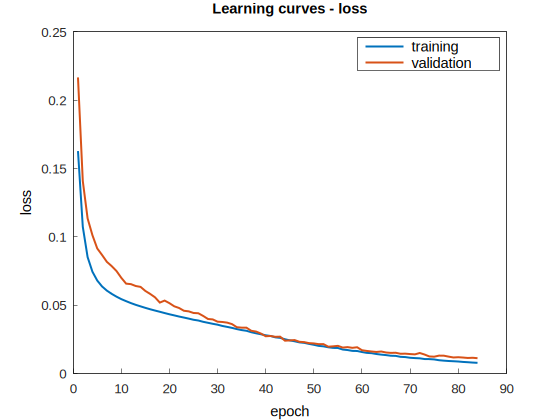
\includegraphics[width=0.49\textwidth]{../img/learning_loss.png}
    \hfill
    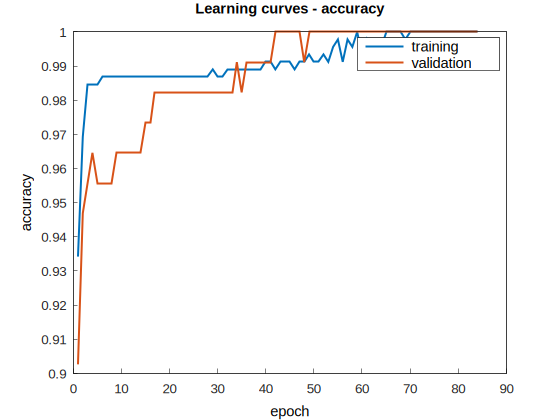
\includegraphics[width=0.49\textwidth]{../img/learning_accuracy.png}
    \caption{Функция потерь и доля правильных ответов по эпохам}
    \label{fig:curves}
\end{figure}

Обе кривые функции потерь монотонно убывают и сближаются по ходу обучения. Динамика
разрыва между ними приведена в таблице~\ref{tab:gap}.

\begin{table}[htbp]
\caption{Функция потерь по эпохам и разрыв между выборками}
\label{tab:gap}
\begin{center}
\begin{tabular}{|r|r|r|r|}
\hline
Эпоха & $L$ & $L_{\text{val}}$ & Разрыв \\
\hline
 1 & 0,1628 & 0,2167 & 0,0539 \\
12 & 0,0515 & 0,0654 & 0,0139 \\
24 & 0,0401 & 0,0454 & 0,0053 \\
36 & 0,0312 & 0,0335 & 0,0023 \\
48 & 0,0224 & 0,0229 & 0,0005 \\
60 & 0,0157 & 0,0170 & 0,0013 \\
72 & 0,0110 & 0,0150 & 0,0039 \\
84 & 0,0077 & 0,0111 & 0,0034 \\
\hline
\end{tabular}
\end{center}
\end{table}

Разрыв сокращается с 0,0539 на первой эпохе до 0,0034 на последней, то
есть признаков переобучения нет. Наилучшей по функции потерь на проверочной выборке
оказывается последняя, 84-я эпоха, поэтому ранняя остановка в итоговом запуске не
срабатывает. Доля правильных ответов на проверочной выборке достигает единицы на 42-й
эпохе, после чего продолжает убывать только функция потерь.

\section{Итоговое качество}

Результат прогноза на проверочной выборке из 113 примеров при зерне 42 приведён в
таблице~\ref{tab:final}.

\begin{table}[htbp]
\caption{Качество итоговой модели и матрица ошибок на проверочной выборке}
\label{tab:final}
\begin{center}
\begin{tabular}{|l|r|r|}
\hline
Бинарная кросс-энтропия & \multicolumn{2}{c|}{0,0111} \\
Доля правильных ответов & \multicolumn{2}{c|}{1,0000} \\
\hline
 & Прогноз B & Прогноз M \\
\hline
Фактически B & 71 & 0 \\
Фактически M & 0 & 42 \\
\hline
\end{tabular}
\end{center}
\end{table}

